% Provenance (never printed): see sources/outline_sources.md (Year 1: decay systems K-Ar,
% Rb-Sr, U-Pb and radiocarbon; closure temperature; dating sedimentary sequences with
% volcanic ashes; calibrating the scale). Exercise and problem values in the Book 3
% scratch calculator calc/ch25.py; figures from figdata/bachelor-1/decay_curves.py,
% isochron.py and radiocarbon.py (IntCal20, dataset bachelor-1-intcal20).
% The decay law, half-life and decay constant belong to the physics series (recalled);
% the closed system and the isochron of minerals are Book 2's (g12 age-of-the-earth),
% re-founded here with whole-rock samples and least squares. The concordia diagram and
% thermochronology are the Year 3 volume's: prose pointers only. Mass spectrometry is
% the chemistry series' (recalled). The isochron figure uses an invented rhyolite so that
% the Varden granite of the problem is not solved in the course.
\chapter{Radiometrische dateringsmethoden}\label{ch:b1:radiometric-methods}

In 2001 rapporteerde een team dat werkte aan detritische zirkoonkorrels uit de Jack Hills in West-Australië er één die
\num[uncertainty-mode=separate]{4404 \pm 8} miljoen jaar geleden was gekristalliseerd. Later werk bevestigde de leeftijd van deze korrels: het zijn het oudste bekende materiaal van enige soort dat op de aarde is gevormd, en zij tonen dat een \omterm{def:b1:layered-earth:layers}{korst} zich binnen ongeveer 160 miljoen jaar na de geboorte van het zonnestelsel had gevormd. Aan het andere uiteinde van de schaal hebben argonleeftijden de extinctie aan het einde van het Krijt, \qty{66.00}{\Ma} geleden, geplaatst binnen \num{32000} jaar van de inslag waarvan wordt gedacht dat hij haar veroorzaakte. Beide getallen komen van het tellen van atomen: een radioactieve ouder die vervalt met een bekende snelheid, een dochter die zich ophoopt. Dit hoofdstuk legt uit hoe zulke klokken worden afgelezen, waarom elk een andere gebeurtenis dateert, en hoe zij de schaal van \cref{ch:b1:stratigraphic-scale} aan een schaal van jaren hangen.
% ledger: wilde01:4404, uw14:jack-hills, ics:base.Paleogene, renne:kpg

\begin{omfigure}
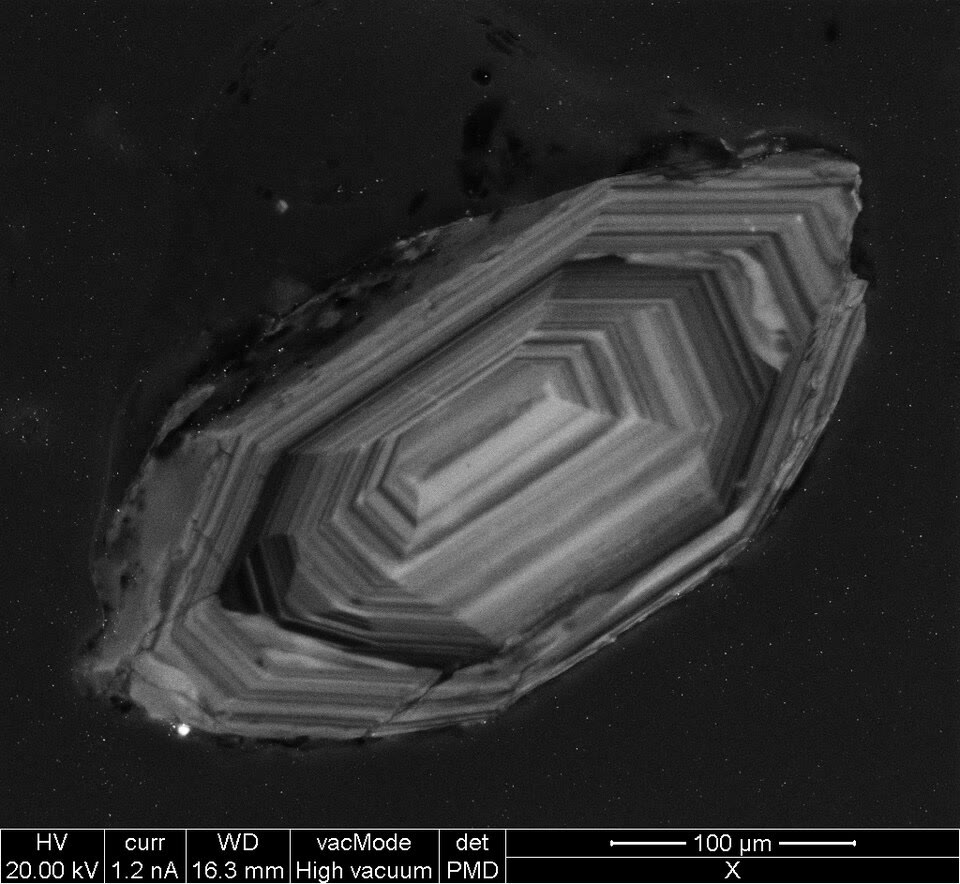
\includegraphics[width=0.5\linewidth]{images/book3/b1-zircon-cl.jpg}

{\small Een korrel zirkoon, ongeveer een derde millimeter lang, afgebeeld door het licht dat zij uitzendt onder de elektronenbundel van een scanning-elektronenmicroscoop (kathodoluminescentie). De banden die de vlakken van het kristal volgen, zijn zones van iets verschillende samenstelling, die na elkaar werden afgezet terwijl zij groeide. Deze korrel werd uit een zandsteen gehaald, dus is zij ouder dan de zandsteen: zij dateert het gesteente waaruit zij werd geërodeerd. (Emmanuel Roquette, CC~BY-SA~4.0, via Wikimedia Commons.)}
\label{fig:b1:radiometric-methods:zircon}
\end{omfigure}
% ledger: commons:zircon-cl

\begin{recall}
De natuurkundeboeken beschrijven radioactief verval: de kernen van een radioactief isotoop vervallen op willekeurige momenten, onafhankelijk van temperatuur en druk, zodat het aantal $N$ dat na een tijd $t$ overblijft $N = N_0\,e^{-\lambda t}$ volgt, waarin $\lambda$ de vervalconstante is; de halveringstijd is $T = \ln 2/\lambda$. Isotopen van een element hebben hetzelfde aantal protonen en een verschillend aantal neutronen; de scheikundeboeken beschrijven de massaspectrometer, die ionen op massa sorteert. In Boek~2, klas~12, is een gesteente of \omterm{def:b1:rock-forming-minerals:mineral}{mineraal} dat geen moeder- of dochteratomen met zijn omgeving heeft uitgewisseld een gesloten systeem, en de mineralen van de Varden-graniet, uitgezet op een rubidium--strontium-isochroon, gaven een leeftijd van 310 miljoen jaar. Biotiet, muscoviet en hoornblende zijn de \omterm{def:b1:rock-forming-minerals:groups}{micas} en het \omterm{def:b1:rock-forming-minerals:groups}{amfibool} van \cref{def:b1:rock-forming-minerals:groups}. Een leeftijd tussen twee gedateerde niveaus kan worden geïnterpoleerd (\cref{prop:b1:stratigraphic-scale:interpolation}).
\end{recall}
% ledger: tulane:radiometric, villa22:rb87

\section{Vervalsystemen}\label{sec:b1:radiometric-methods:systems}

Een klok heeft twee tellingen nodig: wat van de ouder is overgebleven, en hoeveel dochter zij sinds de start van de klok heeft gevormd.

\begin{definition}[Moederisotoop, radiogene dochter]\label{def:b1:radiometric-methods:radiogenic}
In een vervalsysteem dat voor datering wordt gebruikt, is de \emph{moederisotoop}\index{moederisotoop} het radioactieve isotoop waarvan het verval als klok dient, en de dochter is het isotoop dat het verval voortbrengt. De \emph{radiogene
dochter}\index{radiogene dochter}, geschreven $D^*$, is het deel van de dochter dat door het verval van de moeder binnen het monster is gemaakt sinds de klok begon; het overige, $D_0$, was er van het begin af. Het aantal atomen van de dochter dat vandaag wordt gemeten, is $D = D_0 + D^*$.
\end{definition}

\begin{proposition}[Radiogene aanwas en de leeftijdsvergelijking]\label{prop:b1:radiometric-methods:growth}
In een gesloten systeem dat vandaag $P$ atomen van de moeder bevat, is de \omterm{def:b1:radiometric-methods:radiogenic}{radiogene
dochter} die in een tijd $t$ is gemaakt
\[
  D^* = P\,\bigl(e^{\lambda t} - 1\bigr),
\]
op voorwaarde dat elk verval één atoom van de dochter geeft. De leeftijd is dan
\[
  t = \frac{1}{\lambda}\,\ln\!\left(1 + \frac{D^*}{P}\right).
\]
\end{proposition}

\begin{proof}
Volgens de vervalwet was de moeder bij de start van de klok $P_0 = P\,e^{\lambda t}$ groot.
In een gesloten systeem is elk ontbrekend moederatoom een dochteratoom geworden, dus $D^* = P_0 - P = P\,(e^{\lambda t} - 1)$. Dan geldt $e^{\lambda t} = 1 +
D^*/P$; logaritmen nemen geeft de leeftijd.
\end{proof}

De leeftijd hangt alleen af van een verhouding van twee aantallen atomen, wat een massaspectrometer het best meet. De figuur hieronder toont de twee tellingen in eenheden van de halveringstijd: na één halveringstijd is $D^*/P = 1$, na twee $3$, na drie $7$ --- in het algemeen $2^n - 1$ na $n$ halveringstijden.

\begin{omfigure}
\begin{tikzpicture}
\begin{axis}[omrecord, width=0.72\linewidth, height=5.6cm, xmin=0, xmax=5, ymin=0, ymax=1.05,
  xlabel={tijd (halveringstijden)}, ylabel={fractie van de aanvankelijke moeder},
  xtick={0,1,...,5}, ytick={0,0.25,0.5,0.75,1}]
% computed in figdata/bachelor-1/decay_curves.py (no real-world number)
\addplot[omThm, line width=1pt] table[x=n, y=P] {figdata/out/bachelor-1-decay_curves-curves.dat};
\addplot[omDef, line width=1pt] table[x=n, y=D] {figdata/out/bachelor-1-decay_curves-curves.dat};
\addplot[only marks, mark=*, mark size=1.4pt, black!60] table[x=n, y=P] {figdata/out/bachelor-1-decay_curves-marks.dat};
\addplot[only marks, mark=*, mark size=1.4pt, black!60] table[x=n, y=D] {figdata/out/bachelor-1-decay_curves-marks.dat};
\node[font=\small, text=omThm, anchor=south west] at (axis cs:0.35,0.80) {moeder $P$};
\node[font=\small, text=omDef, anchor=north west] at (axis cs:2.55,0.66) {radiogene dochter $D^*$};
\node[font=\scriptsize, anchor=west, inner sep=1pt] (r1) at (axis cs:0.12,0.5) {$D^*/P = 1$};
\draw[black!60, line width=0.4pt] (r1.east) -- (axis cs:0.95,0.5);
\node[font=\scriptsize, anchor=south] at (axis cs:2,0.77) {$3$};
\node[font=\scriptsize, anchor=south] at (axis cs:3,0.89) {$7$};
\node[font=\scriptsize, anchor=north] at (axis cs:4,0.915) {$15$};
\node[font=\scriptsize, anchor=north east] at (axis cs:4.97,0.95) {$31$};
\end{axis}
\end{tikzpicture}

{\small De moeder en haar \omterm{def:b1:radiometric-methods:radiogenic}{radiogene dochter} in een gesloten systeem, als fracties van het aanvankelijke aantal moederatomen, tegen de tijd geteld in halveringstijden. Hun som blijft gelijk aan één; de verhouding $D^*/P$, bij elke hele halveringstijd vermeld, verdubbelt en telt bij elke stap één op.}
\label{fig:b1:radiometric-methods:decay}
\end{omfigure}

Een klok leest alleen goed binnen een venster van leeftijden. Lang vóór één halveringstijd is de dochter een klein deel van de moeder; na vele halveringstijden is er te weinig moeder over om te meten. De tabel hieronder somt de meest gebruikte systemen op, met het materiaal waarop elk wordt toegepast.

\begin{table}[ht]
\centering
\small
\renewcommand{\arraystretch}{1.25}
\begin{tabular}{|l|l|c|c|>{\raggedright\arraybackslash}p{4.3cm}|}
\hline
moeder & dochter & halveringstijd (jaar) & $\lambda$ (per jaar) & gedateerd materiaal \\
\hline
$^{14}\mathrm{C}$ & $^{14}\mathrm{N}$ & \num{5700} & \num{1.216e-4} & hout, houtskool, been, schelp \\
$^{40}\mathrm{K}$ & $^{40}\mathrm{Ar}$, $^{40}\mathrm{Ca}$ & \num{1.25e9} & \num{5.543e-10} & kaliumrijke mineralen: sanidien, biotiet, hoornblende \\
$^{87}\mathrm{Rb}$ & $^{87}\mathrm{Sr}$ & \num{4.96e10} & \num{1.3972e-11} & graniet (hele gesteenten), \omterm{def:b1:rock-forming-minerals:groups}{micas} \\
$^{147}\mathrm{Sm}$ & $^{143}\mathrm{Nd}$ & \num{1.07e11} & \num{6.46e-12} & gesteenten en hun mineralen (isochronen) \\
$^{235}\mathrm{U}$ & $^{207}\mathrm{Pb}$ & \num{7.04e8} & \num{9.8485e-10} & zirkoon \\
$^{238}\mathrm{U}$ & $^{206}\mathrm{Pb}$ & \num{4.47e9} & \num{1.55125e-10} & zirkoon \\
\hline
\end{tabular}
\caption{De voornaamste vervalsystemen. De vervalconstanten van kalium-40 en van de twee uranium-isotopen zijn de conventionele waarden die worden gebruikt om leeftijden te berekenen; die van rubidium-87 en samarium-147 zijn berekend uit de halveringstijden, die van koolstof-14 uit zijn halveringstijd van \num{5700} jaar.}
\label{tab:b1:radiometric-methods:systems}
\end{table}
% ledger: iaea:c14, iaea:k40-branches, amherst:constants, villa22:rb87, iaea:sm147, iaea:isotopes, tulane:kar, tulane:upb-zircon, tulane:c14

Voor dezelfde kernen zijn twee reeksen getallen in gebruik, en een leeftijd moet zeggen welke zij gebruikte. Kerntabellen geven kalium-40 een halveringstijd van \num{1.248e9} jaar en sturen \qty{10.72}{\percent} van zijn vervallen naar argon; de in de geochronologie conventioneel gebruikte constanten geven $\lambda = \num{5.543e-10}$ per jaar (een halveringstijd van \num{1.2505e9}
jaar) en sturen $0.581/5.543 = \qty{10.48}{\percent}$ van de vervallen naar argon. \omterm{def:b1:radiometric-methods:radiocarbon}{Radiokoolstofleeftijden}, zoals \cref{sec:b1:radiometric-methods:kar} uitlegt, worden berekend met een halveringstijd van \num{5568} jaar, waarvan bekend is dat hij te kort is. De verschillen bereiken enkele procenten, veel meer dan de \qty{0.01}{\percent} waarop de beste leeftijden nu worden opgegeven (\cref{sec:b1:radiometric-methods:sediments}). De onzekerheid van de vervalconstanten van kalium-40 zelf, een kern met twee vertakkingen en een lange halveringstijd, beperkt de nauwkeurigheid van zijn leeftijden.
% ledger: iaea:k40-branches, amherst:constants, sp77:conventional-age, ics:base.Triassic, nmgrl:arar

\begin{proposition}[Precisie van een leeftijd]\label{prop:b1:radiometric-methods:precision}
Als de verhouding $R = D^*/P$ wordt gemeten met de standaardonzekerheid $\sigma_R$, draagt de leeftijd de onzekerheid
\[
  \sigma_t = \frac{\sigma_R}{\lambda\,(1 + R)}.
\]
\end{proposition}

\begin{proof}
Voor een kleine fout $\delta R$ verandert de leeftijd $t = \ln(1+R)/\lambda$ met
$\delta t = t'(R)\,\delta R = \delta R/\bigl(\lambda(1 + R)\bigr)$.
\end{proof}

Voor een jong monster is $R$ klein en $\sigma_t \approx \sigma_R/\lambda$: de absolute fout van de leeftijd wordt bepaald door hoe goed een kleine hoeveelheid dochter kan worden gemeten. Een lange halveringstijd (kleine $\lambda$) vergroot haar. Daarom dienen rubidium--strontium en uranium--lood voor gesteenten die ouder zijn dan ongeveer tien miljoen jaar, terwijl kalium--argon reikt tot gesteenten van ongeveer tien duizend jaar, en radiokoolstof de laatste \num{70000} jaar bestrijkt.
% ledger: tulane:ranges

\section{Isochronen}\label{sec:b1:radiometric-methods:isochrons}

De leeftijdsvergelijking heeft $D^*$ nodig, maar het instrument meet $D = D_0 + D^*$, en
$D_0$ is zelden nul: strontium-87 is aanwezig in elk \omterm{def:b1:rock-forming-minerals:mineral}{mineraal} dat bij zijn vorming strontium opnam. De \omterm{def:b1:radiometric-methods:isochron}{isochroon} verwijdert $D_0$ door verschillende monsters te meten die met dezelfde isotopensamenstelling van het dochterelement begonnen.

\begin{definition}[Isochroon, beginverhouding]\label{def:b1:radiometric-methods:isochron}
Laat $S$ een stabiel isotoop van het dochterelement zijn dat door geen verval wordt geproduceerd ($^{86}\mathrm{Sr}$ voor strontium, $^{144}\mathrm{Nd}$ voor neodymium). Een \emph{isochroon}\index{isochroon} is de rechte lijn waarop, in een grafiek van $y = D/S$ tegen $x = P/S$, monsters liggen die tegelijk zijn gevormd met dezelfde waarde van $D/S$ en sindsdien gesloten systemen zijn geweest. Die gedeelde beginwaarde $y_0 = (D/S)_0$ is de \emph{beginverhouding}\index{beginverhouding}.
\end{definition}
% ledger: tulane:radiometric, tulane:c14

\begin{theorem}[De isochroon]\label{thm:b1:radiometric-methods:isochron}
Monsters die tegelijk zijn gevormd met dezelfde \omterm{def:b1:radiometric-methods:isochron}{beginverhouding} $y_0$, en die gedurende een tijd $t$ gesloten systemen zijn geweest, voldoen aan
\[
  y = y_0 + \bigl(e^{\lambda t} - 1\bigr)\,x .
\]
Hun punten liggen op een rechte lijn met helling $m = e^{\lambda t} - 1$ en snijpunt $y_0$, en $t = \ln(1+m)/\lambda$.
\end{theorem}

\begin{proof}
Voor elk monster geldt $D = D_0 + P\,(e^{\lambda t} - 1)$ volgens
\cref{prop:b1:radiometric-methods:growth}. Het aantal atomen van $S$ is niet veranderd, omdat $S$ stabiel is, door geen verval wordt gemaakt en het systeem gesloten is; het delen daardoor geeft $y = y_0 + (e^{\lambda t} - 1)\,x$, met $y_0$ voor alle monsters dezelfde volgens de hypothese.
\end{proof}

Toen een graniet kristalliseerde, hadden al zijn monsters dezelfde $y_0$ en lagen zij op een horizontale lijn; elk is sindsdien omhoog bewogen in verhouding tot zijn $x$, en de lijn is rond haar snijpunt gedraaid. De monsters hebben verschillende waarden van $x$ nodig om de helling goed te bepalen: mineralen met veel en weinig rubidium, zoals in Boek~2, of gesteentemonsters die uit meer en minder geëvolueerde delen van één intrusie zijn genomen. Een punt naast de lijn markeert een monster dat niet gesloten was, of de gedeelde \omterm{def:b1:radiometric-methods:isochron}{beginverhouding} niet deelde. De \omterm{def:b1:radiometric-methods:isochron}{beginverhouding} is zelf een tracer: een magma uit de \omterm{def:b1:layered-earth:layers}{mantel} erft een lage $^{87}\mathrm{Sr}/^{86}\mathrm{Sr}$, ongeveer $0.7025$, en een magma uit gesmolten continentale \omterm{def:b1:layered-earth:layers}{korst} een hoge, ongeveer $0.710$, omdat de \omterm{def:b1:layered-earth:layers}{korst} rijk is aan rubidium en in de loop der tijden meer strontium-87 heeft gemaakt.
% ledger: tulane:radiometric, tulane:sr-initial

Echte punten vallen nooit precies op een lijn. De gebruikelijke schatting van de lijn is die welke de gekwadrateerde verticale afstanden van de punten tot haar zo klein mogelijk maakt.

\begin{proposition}[De kleinste-kwadratenlijn]\label{prop:b1:radiometric-methods:lsq}
Laat $(x_i, y_i)$, $i = 1, \dots, n$, punten zijn met ten minste twee verschillende $x_i$,
met gemiddelden $\bar x$ en $\bar y$, en laat
\[
  S_{xx} = \sum_i (x_i - \bar x)^2, \qquad S_{xy} = \sum_i (x_i - \bar x)(y_i - \bar y).
\]
De lijn $y = b + m x$ die $Q(b, m) = \sum_i (y_i - b - m x_i)^2$ minimaliseert, heeft
\[
  m = \frac{S_{xy}}{S_{xx}}, \qquad b = \bar y - m\,\bar x ,
\]
en gaat door het zwaartepunt $(\bar x, \bar y)$.
\end{proposition}

\begin{proof}
$Q$ is een som van kwadraten, een polynoom van graad twee in $(b, m)$ dat in elke richting naar oneindig gaat, dus bereikt het zijn minimum waar beide partiële afgeleiden nul zijn. $\partial Q/\partial b = -2 \sum_i (y_i - b - m x_i) = 0$ geeft $n\bar y = n b + n m \bar x$, dus $b = \bar y - m \bar x$: de lijn gaat door het zwaartepunt. Invullen geeft $y_i - b - m x_i = (y_i - \bar y) - m(x_i -
\bar x)$, en $\partial Q/\partial m = -2 \sum_i x_i \bigl[(y_i - \bar y) - m(x_i
- \bar x)\bigr] = 0$. Aangezien $\sum_i (y_i - \bar y) = \sum_i (x_i - \bar x) = 0$, mag $x_i$
in deze som worden vervangen door $x_i - \bar x$, wat $S_{xy} - m S_{xx} = 0$ geeft.
$S_{xx} > 0$ omdat de $x_i$ niet allemaal gelijk zijn.
\end{proof}

De spreiding van de punten rond de lijn geeft de onzekerheid van de helling. Met de residuen $r_i = y_i - b - m x_i$ is de standaardafwijking van de spreiding $s = \sqrt{\sum_i r_i^2/(n-2)}$ --- twee vrijheidsgraden worden gebruikt door de twee parameters --- en zijn de standaardonzekerheden van de helling en van het snijpunt
\[
  \sigma_m = \frac{s}{\sqrt{S_{xx}}}, \qquad
  \sigma_b = s\,\sqrt{\frac1n + \frac{\bar x^2}{S_{xx}}} .
\]
Deze twee resultaten van de statistiek worden hier aangenomen; de leeftijd draagt dan $\sigma_t = \sigma_m/\bigl(\lambda(1 + m)\bigr)$, volgens het argument van \cref{prop:b1:radiometric-methods:precision}. Zij tonen wat een goede \omterm{def:b1:radiometric-methods:isochron}{isochroon} maakt: veel punten, breed verspreid in $x$ (een grote $S_{xx}$), met weinig spreiding.

\begin{method}[Een isochroon passen]\label{met:b1:radiometric-methods:isochron}
\begin{enumerate}
  \item Meet $x = P/S$ en $y = D/S$ in ten minste vier monsters van één lichaam, zo gekozen dat $x$ zo breed mogelijk wordt gespreid.
  \item Zet ze uit; leg elk punt dat duidelijk naast de trend ligt terzijde, met een reden.
  \item Bereken $\bar x$, $\bar y$, $S_{xx}$, $S_{xy}$, dan $m = S_{xy}/S_{xx}$
        en $b = \bar y - m \bar x$.
  \item Bereken de residuen, $s$, $\sigma_m$ en $\sigma_b$.
  \item De leeftijd is $t = \ln(1+m)/\lambda$, met $\sigma_t =
        \sigma_m/\bigl(\lambda(1+m)\bigr)$; de \omterm{def:b1:radiometric-methods:isochron}{beginverhouding} is $b \pm \sigma_b$.
\end{enumerate}
\end{method}

\begin{example}[Een verzonnen rhyoliet]\label{ex:b1:radiometric-methods:rhyolite}
Zes gesteentemonsters van een reeks rhyolietlava's (oefengegevens) geven:
\begin{center}
\small
\begin{tabular}{|l|cccccc|}
\hline
$x = {}^{87}\mathrm{Rb}/^{86}\mathrm{Sr}$ & 1.85 & 4.62 & 9.30 & 14.75 & 21.20 & 27.60 \\
$y = {}^{87}\mathrm{Sr}/^{86}\mathrm{Sr}$ & 0.71732 & 0.73332 & 0.76164 & 0.79420 & 0.83226 & 0.87028 \\
\hline
\end{tabular}
\end{center}
Hier is $\bar x = 13.22$, $\bar y = 0.784837$, $S_{xx} = 491.41$ en
$S_{xy} = 2.92308$, dus $m = 0.0059484$ en $b = 0.70620$. De residuen geven
$s = 0.00024$, $\sigma_m = \num{1.10e-5}$ en $\sigma_b = 0.00018$. De leeftijd is
$t = \ln(1.0059484)/\num{1.3972e-11} = \qty{424.5}{\Ma}$, met
$\sigma_t = \num{1.10e-5}/(\num{1.3972e-11} \times 1.0059) = \qty{0.8}{\Myr}$:
\qty[uncertainty-mode=separate]{424.5(8)}{\Ma}, \omterm{def:b1:radiometric-methods:isochron}{beginverhouding}
\num[uncertainty-mode=separate]{0.70620(18)} (figuur hieronder).
\end{example}
% values: isochron.py (slope 0.005948361, intercept 0.7061993, age 424.4732, sigma 0.7827871); ledger: villa22:rb87

\begin{omfigure}
\begin{tikzpicture}
\begin{axis}[omrecord, width=0.74\linewidth, height=6cm, xmin=0, xmax=30, ymin=0.70, ymax=0.88,
  xlabel={$^{87}\mathrm{Rb}/^{86}\mathrm{Sr}$}, ylabel={$^{87}\mathrm{Sr}/^{86}\mathrm{Sr}$},
  ytick={0.70,0.72,...,0.88},
  y tick label style={/pgf/number format/.cd, fixed, fixed zerofill, precision=2}]
% computed in figdata/bachelor-1/isochron.py (exercise data, invented rhyolite); ledger: villa22:rb87
\addplot[black!60, densely dotted, line width=0.7pt] table[x=x, y=y] {figdata/out/bachelor-1-isochron-initial.dat};
\addplot[omDef, line width=0.9pt] table[x=x, y=y] {figdata/out/bachelor-1-isochron-line.dat};
\addplot[omThm, only marks, mark=*, mark size=2pt] table[x=x, y=y] {figdata/out/bachelor-1-isochron-points.dat};
\node[font=\scriptsize, text=omDef, anchor=south east, align=right] at (axis cs:19,0.83)
  {kleinstekwadratenhelling $0.005948$\\ leeftijd \qty[uncertainty-mode=separate]{424.5(8)}{\Ma}};
\node[font=\scriptsize, text=black!70, anchor=south west] at (axis cs:9,0.7068)
  {beginverhouding $0.70620$, toen de lavastromen zich vormden};
\end{axis}
\end{tikzpicture}

{\small Een rubidium--strontium-isochroon van zes gesteentemonsters van een verzonnen rhyoliet (oefengegevens). De punten verstrooien zich enigszins rond de kleinste-kwadratenlijn, die door hun zwaartepunt gaat; de gestippelde lijn is waar zij allemaal lagen toen de lavastromen zich vormden.}
\label{fig:b1:radiometric-methods:isochron}
\end{omfigure}

\begin{inthelab}[Isotopen wegen]
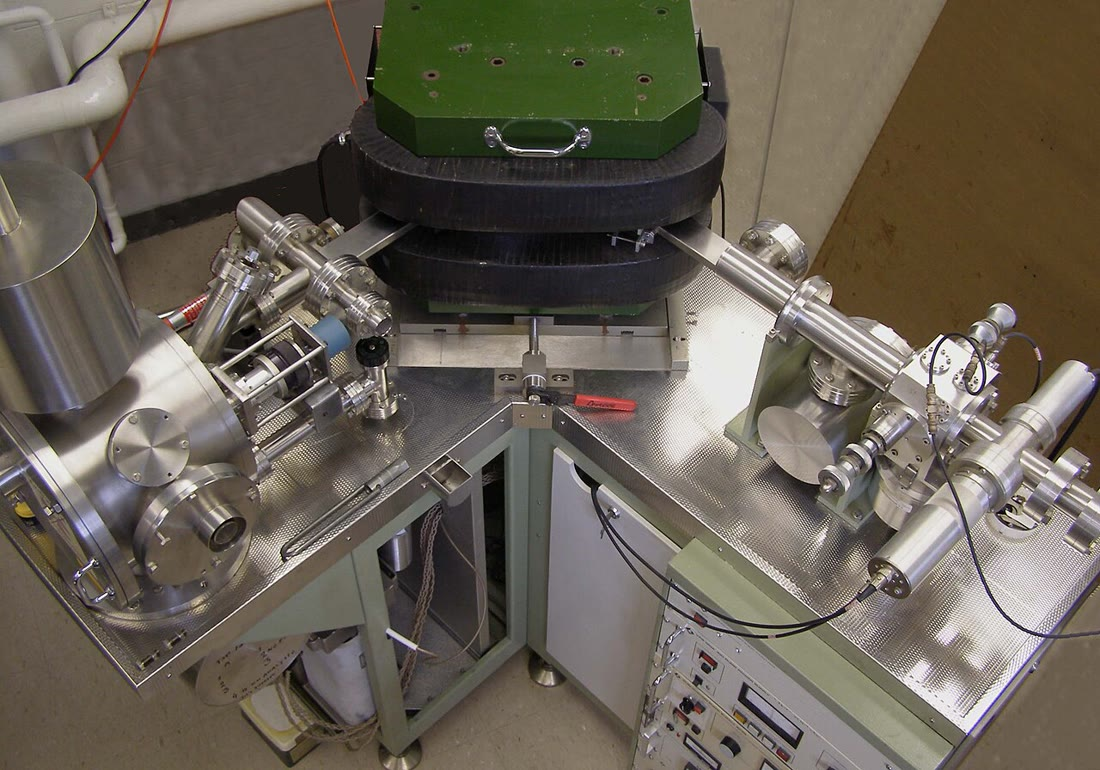
\includegraphics[width=0.42\linewidth]{images/book3/b1-tims.jpg}\hfill
\begin{minipage}[b]{0.55\linewidth}
Een thermische-ionisatiemassaspectrometer (links) meet de isotopenverhoudingen van elementen zoals strontium. Het element, door scheikunde uit het opgeloste monster afgescheiden, wordt op een metalen draad in vacuüm geladen; verhit geeft het ionen af, die worden versneld en gebogen door het veld van de grote elektromagneet (de zwarte spoelen in het midden), lichtere ionen meer dan zwaardere, zodat elk isotoop zijn eigen verzamelaar bereikt. Verhoudingen van isotopen zijn wat het instrument het best meet, en daarom zijn methoden die alleen op verhoudingen steunen het nauwkeurigst.
(Foto: Radiogenic, CC0, via Wikimedia Commons.)
\end{minipage}
\end{inthelab}
% ledger: commons:tims, amherst:constants

\section{Kalium--argon, uranium--lood en radiokoolstof}\label{sec:b1:radiometric-methods:kar}

\subsection*{Een moeder met twee dochters}

\begin{definition}[Vertakkend verval]\label{def:b1:radiometric-methods:branching}
Een moeder ondergaat \emph{vertakkend verval}\index{vertakkend verval} wanneer haar kernen via twee of meer routes naar verschillende dochters vervallen. Elke route $i$ heeft haar eigen gedeeltelijke vervalconstante $\lambda_i$; de moeder vervalt met de totale constante $\lambda = \sum_i \lambda_i$, en een fractie $\lambda_i/\lambda$ van de vervallen neemt route~$i$. Kalium-40 vervalt tot calcium-40 met $\lambda_\beta =
\num{4.962e-10}$ per jaar en tot argon-40 met $\lambda_e = \num{0.581e-10}$ per
jaar.
\end{definition}
% ledger: amherst:constants, iaea:k40-branches

\begin{proposition}[De kalium-argonleeftijd]\label{prop:b1:radiometric-methods:kar}
Een \omterm{def:b1:rock-forming-minerals:mineral}{mineraal} dat al het argon dat erin is gemaakt heeft behouden, en geen argon bevatte toen het vormde, bevat na een tijd $t$
\[
  {}^{40}\mathrm{Ar}^* = \frac{\lambda_e}{\lambda}\;{}^{40}\mathrm{K}\,\bigl(e^{\lambda t} - 1\bigr),
  \qquad\text{dus}\qquad
  t = \frac{1}{\lambda}\,\ln\!\left(1 + \frac{\lambda}{\lambda_e}\,
      \frac{{}^{40}\mathrm{Ar}^*}{{}^{40}\mathrm{K}}\right),
\]
waarin ${}^{40}\mathrm{K}$ het aantal kalium-40-atomen vandaag is en $\lambda =
\lambda_\beta + \lambda_e$.
\end{proposition}

\begin{proof}
De moeder vervalt met de totale constante $\lambda$, wat de route ook is, dus is volgens
\cref{prop:b1:radiometric-methods:growth} het aantal vervallen in de tijd $t$
${}^{40}\mathrm{K}\,(e^{\lambda t} - 1)$. Elk verval neemt de argonroute met kans $\lambda_e/\lambda$, onafhankelijk van de andere; over het zeer grote aantal vervallen is de fractie die argon gaf $\lambda_e/\lambda$. Dit geeft ${}^{40}\mathrm{Ar}^*$; het oplossen naar $t$ geeft de leeftijd.
\end{proof}

De exponent bevat de totale constante en de factor ervoor de gedeeltelijke: het gebruik van $\lambda_e$ in de exponent, alsof argon de enige route was, zou een volkomen foute leeftijd geven. De calciumtak draagt negen tiende van de vervallen, maar is nutteloos voor datering, omdat calcium-40 het gewone isotoop is van een element dat in gesteenten overvloedig voorkomt; argon, een edelgas, ontsnapt uit een smelt, zodat een kristal vrijwel zonder argon begint. Kalium-40 is \qty{0.0117}{\percent} van de atomen van kalium. De methode heeft de absolute hoeveelheden van zowel kalium als argon nodig, apart gemeten. Argon uit de lucht, in elk gesteente aanwezig, wordt herkend aan zijn argon-36 en afgetrokken met de atmosferische verhouding
$^{40}\mathrm{Ar}/^{36}\mathrm{Ar} = 295.5$.
% ledger: tulane:kar, iaea:k40-branches, amherst:constants, nmgrl:kar

De methode faalt op twee manieren. Overtollig argon maakt leeftijden te oud: een lava die snel afkoelt, kan argon uit de \omterm{def:b1:layered-earth:layers}{mantel} in bellen vangen, en historische lava's geven gewoonlijk kalium--argonleeftijden van 1 tot 2 miljoen jaar, een fout die alleen voor jonge gesteenten telt. Argonverlies maakt ze te jong: de meeste mineralen verliezen argon bij verhitting boven ongeveer \qty{300}{\celsius}, zodat een latere metamorfose de klok geheel of gedeeltelijk reset, en een gedeeltelijk verlies geeft een leeftijd tussen de twee gebeurtenissen die geen van beide dateert. Kaliumrijke mineralen hebben de voorkeur: sanidien en biotiet, dan \omterm{def:b1:rock-forming-minerals:groups}{plagioklaas} of hoornblende.
% ledger: tulane:kar, nmgrl:kar

De argon--argonmethode meet alleen verhoudingen. Het monster wordt bestraald met snelle neutronen in de kern van een kernreactor, naast een standaardmineraal van bekende leeftijd; de reactie zet een deel van zijn kalium-39 om in argon-39, dat dan voor het kalium staat, en de standaard geeft het rendement van de reactie. De twee isotopen worden samen in hetzelfde gas gemeten. Het monster kan dan in stappen worden verhit, met een oven of een laser; elke stap geeft een leeftijd, en de leeftijden worden uitgezet tegen de cumulatieve fractie van vrijgekomen argon-39, een leeftijdsspectrum. Stappen die binnen hun fouten overeenkomen, vormen een plateau; een spectrum zonder plateau waarschuwt dat het \omterm{def:b1:rock-forming-minerals:mineral}{mineraal} niet gesloten is gebleven. De gelijktijdigheid van de inslag en de extinctie aan het einde van het Krijt berust op argon--argonleeftijden.
% ledger: amherst:arar, nmgrl:arar, renne:kpg

\subsection*{Twee uraniumklokken}

Uranium heeft twee langlevende isotopen, uranium-238 dat vervalt tot lood-206 en uranium-235 tot lood-207, tegen verschillende snelheden; vandaag is $^{235}\mathrm{U}/^{238}\mathrm{U} = 0.0072567$, één atoom op 137.8. Een \omterm{def:b1:rock-forming-minerals:mineral}{mineraal} dat uranium bevat, draagt dus twee onafhankelijke klokken, elk met zijn eigen groeivergelijking ${}^{206}\mathrm{Pb}^* = {}^{238}\mathrm{U}\,(e^{\lambda_{238} t} - 1)$ en ${}^{207}\mathrm{Pb}^* = {}^{235}\mathrm{U}\,(e^{\lambda_{235} t} - 1)$. Als de twee leeftijden overeenkomen, heten zij concordant, en de overeenstemming is een toets dat het \omterm{def:b1:rock-forming-minerals:mineral}{mineraal} gesloten is gebleven, wat geen enkele klok alleen kan geven. Onenigheid komt vooral van lood dat is verloren uit delen van het kristal die door de straling van het uranium zelf zijn beschadigd; een grafiek van de twee verhoudingen tegen elkaar, het concordiadiagram, herstelt dan zowel de leeftijd van het kristal als die van de gebeurtenis die het lood deed verliezen --- een hulpmiddel van Boek~5.
% ledger: amherst:constants, tulane:upb-zircon

Zirkoon, $\mathrm{ZrSiO_4}$, is het \omterm{def:b1:rock-forming-minerals:mineral}{mineraal} van keuze: het neemt uranium in zijn structuur op, maar bijna geen lood, zodat bijna al zijn lood radiogeen is; het is hard, weerstaat verwering en overleeft metamorfose, zodat korrels die uit een gesteente zijn geërodeerd hun leeftijd bewaren in de zanden die ervan zijn afgeleid. Apatiet en titaniet worden ook gebruikt, minder vaak.
% ledger: tulane:upb-zircon, commons:zircon-cl

\subsection*{Radiokoolstof}

Koolstof-14 wordt voortdurend in de bovenste atmosfeer gemaakt uit stikstof-14 dat door kosmische straling wordt getroffen. Het voegt zich bij de koolstof van de atmosfeer; levende organismen wisselen koolstof met de atmosfeer uit en houden hun aandeel koolstof-14 op peil. Bij de dood stopt de uitwisseling en vervalt de koolstof-14 terug tot stikstof-14. Omdat het aanvankelijke aandeel dat van de atmosfeer is, volgt de leeftijd uit de vervalwet alleen, zonder \omterm{def:b1:radiometric-methods:isochron}{isochroon}: $t = -\tau \ln(A/A_0)$, waarin $A$ de activiteit is van de koolstof van het monster, $A_0$ die van levende koolstof en $\tau =
1/\lambda$ de gemiddelde levensduur. Hout, houtskool, been, tanden en schelp worden zo gedateerd, tot enkele tienduizenden jaren: ongeveer \num{70000} jaar op zijn hoogst.
% ledger: tulane:c14, iaea:c14

\begin{definition}[Radiokoolstofleeftijd, kalibratiecurve]\label{def:b1:radiometric-methods:radiocarbon}
De (conventionele) \emph{radiokoolstofleeftijd}\index{radiokoolstofleeftijd} van een monster is
\[
  t = -8033 \,\ln \frac{A_{\mathrm{SN}}}{A_{\mathrm{ON}}} \ \text{jaar BP},
\]
waarin $A_{\mathrm{SN}}$ de activiteit is van de koolstof van het monster en $A_{\mathrm{ON}}$ die van de referentiestandaard; zij gebruikt de halveringstijd van \num{5568} jaar (gemiddelde levensduur \num{8033} jaar), normaliseert de activiteiten voor de isotopenfractionering van koolstof ($\delta^{13}\mathrm{C} = \qty{-25}{\permil}$), en telt jaren vóór AD~1950 (BP, ``before present''). Een \emph{kalibratiecurve}\index{kalibratiecurve} geeft de radiokoolstofleeftijd van monsters van bekende kalenderleeftijd; achterwaarts gelezen zet zij een radiokoolstofleeftijd om in een reeks kalenderleeftijden (cal BP).
\end{definition}
% ledger: sp77:conventional-age, reimer20:intcal20

De \omterm{def:b1:radiometric-methods:radiocarbon}{radiokoolstofleeftijd} is om twee redenen geen leeftijd in kalenderjaren. De halveringstijd van \num{5568} jaar, Libby's waarde, die bij conventie is behouden, is korter dan de werkelijke \num{5700} jaar, zodat \omterm{def:b1:radiometric-methods:radiocarbon}{radiokoolstofleeftijden} ongeveer \qty{2.4}{\percent} te kort uitvallen. Belangrijker is dat het aandeel koolstof-14 in de atmosfeer niet constant is geweest. De \omterm{def:b1:radiometric-methods:radiocarbon}{kalibratiecurve} meet beide effecten samen, op archieven die onafhankelijk zijn gedateerd: boomringen tot ongeveer \num{13900} cal BP, en verder, drijvende boomringreeksen, meer- en zeesedimenten, grotafzettingen en koralen, tot \num{55000} cal BP (figuur hieronder).
% ledger: sp77:conventional-age, iaea:c14, reimer20:intcal20

\begin{omfigure}
\begin{tikzpicture}
\begin{axis}[name=main, omrecord, width=0.5\linewidth, height=6cm, xmin=0, xmax=12, ymin=0, ymax=12,
  xlabel={kalenderleeftijd (duizend cal BP)}, ylabel={radiokoolstofleeftijd (duizend BP)},
  xtick={0,2,...,12}, ytick={0,2,...,12}]
% figdata/bachelor-1/radiocarbon.py, IntCal20 (dataset bachelor-1-intcal20); ledger: data:b3-intcal20
\addplot[black!50, dashed, domain=0:12, samples=2] {x};
\addplot[omDef, line width=0.9pt] table[x=cal, y=c14] {figdata/out/bachelor-1-radiocarbon-curve.dat};
\draw[omThm, line width=0.6pt] (axis cs:2.3,2.3) rectangle (axis cs:2.9,2.9);
\node[font=\scriptsize, anchor=east, text=black!60] at (axis cs:8.4,10.4) {gelijke leeftijden};
\node[font=\scriptsize, text=omDef, anchor=north west] at (axis cs:7.4,5.6) {IntCal20};
\end{axis}
\begin{axis}[at={(main.east)}, anchor=west, xshift=2.1cm, omrecord, width=0.38\linewidth, height=6cm,
  xmin=2300, xmax=2900, ymin=2300, ymax=2900, xlabel={kalenderleeftijd (cal BP)}, ylabel={radiokoolstofleeftijd (BP)},
  xtick={2300,2500,2700,2900}, ytick={2300,2500,2700,2900},
  x tick label style={/pgf/number format/.cd, set thousands separator={}},
  y tick label style={/pgf/number format/.cd, set thousands separator={}}]
\addplot[name path=hi, draw=none, forget plot] table[x=cal, y=hi] {figdata/out/bachelor-1-radiocarbon-zoom.dat};
\addplot[name path=lo, draw=none, forget plot] table[x=cal, y=lo] {figdata/out/bachelor-1-radiocarbon-zoom.dat};
\addplot[omDef!25, forget plot] fill between[of=hi and lo];
\addplot[omDef, line width=0.8pt] table[x=cal, y=c14] {figdata/out/bachelor-1-radiocarbon-zoom.dat};
\addplot[omThm, line width=0.6pt, domain=2300:2900, samples=2] {2480};
\draw[omThm, densely dotted] (axis cs:2495,2300) -- (axis cs:2495,2480);
\draw[omThm, densely dotted] (axis cs:2699,2300) -- (axis cs:2699,2480);
\node[font=\scriptsize, text=omThm, anchor=south west] at (axis cs:2310,2485) {$2480$ BP};
\end{axis}
\end{tikzpicture}
{\small Links: de IntCal20-kalibratiecurve over de laatste \num{12000} jaar, \omterm{def:b1:radiometric-methods:radiocarbon}{radiokoolstofleeftijd} tegen kalenderleeftijd; de gestreepte lijn is waar de twee gelijk zouden zijn. Rechts: het kader links vergroot, met de band van één standaardonzekerheid van de curve. Tussen \num{2500} en \num{2700} cal BP is de curve bijna vlak: een \omterm{def:b1:radiometric-methods:radiocarbon}{radiokoolstofleeftijd} van 2480 jaar BP komt overeen met kalenderleeftijden van ongeveer \num{2495} tot \num{2699} cal BP.}
\label{fig:b1:radiometric-methods:intcal}
\end{omfigure}
% ledger: data:b3-intcal20, reimer20:intcal20

Bij \num{2000} cal BP geeft de curve \num[uncertainty-mode=separate]{2070 \pm 14} jaar BP; bij \num{12000} cal BP, \num{10306}: \omterm{def:b1:radiometric-methods:radiocarbon}{radiokoolstofleeftijden} zijn daar \num{1694} jaar jonger dan kalenderleeftijden, veel meer dan de \qty{2.4}{\percent} van de halveringstijd. De curve golft, en waar hij vlak is, komt een \omterm{def:b1:radiometric-methods:radiocarbon}{radiokoolstofleeftijd} overeen met een lange reeks kalenderleeftijden, hoe nauwkeurig de meting ook is.
% ledger: data:b3-intcal20

\begin{dated}{2020}
% ledger: reimer20:intcal20
De curve die voor het noordelijk halfrond wordt gebruikt, is IntCal20, gepubliceerd in 2020. Zij verving IntCal13, met nieuwe gegevens en uitgebreid tot \num{55000} cal BP, met aparte curven voor het zuidelijk halfrond en voor het oppervlaktewater van de oceaan. \omterm{def:b1:radiometric-methods:radiocarbon}{Kalibratiecurven} worden herzien naarmate nieuwe archieven worden gemeten, dus een kalenderleeftijd moet de curve noemen die haar heeft voortgebracht.
\end{dated}

\section{Sluitingstemperatuur}\label{sec:b1:radiometric-methods:closure}

Een \omterm{def:b1:rock-forming-minerals:mineral}{mineraal} dat uit een magma kristalliseert bij \qty{800}{\celsius}, start zijn klok niet meteen. Terwijl het heet is, diffunderen atomen van de dochter --- vooral argon --- door zijn rooster en ontsnappen; pas wanneer het voldoende is afgekoeld, wordt de diffusie te traag om ertoe te doen, en begint de dochter zich op te hopen.
% ledger: leeds:closure, tulane:kar, tulane:magma-types

\begin{definition}[Sluitingstemperatuur, afkoelingsleeftijd]\label{def:b1:radiometric-methods:closure}
De \emph{sluitingstemperatuur}\index{sluitingstemperatuur} van een \omterm{def:b1:rock-forming-minerals:mineral}{mineraal} voor een vervalsysteem is de temperatuur waaronder de moeder- en dochteratomen niet langer snel genoeg in of uit zijn rooster diffunderen om ertoe te doen, zodat het \omterm{def:b1:rock-forming-minerals:mineral}{mineraal} zich als een gesloten systeem gedraagt. Een \emph{afkoelingsleeftijd}\index{afkoelingsleeftijd} is een leeftijd die is gemeten in een \omterm{def:b1:rock-forming-minerals:mineral}{mineraal} dat boven zijn sluitingstemperatuur is gevormd: zij dateert het moment waarop het \omterm{def:b1:rock-forming-minerals:mineral}{mineraal} door die temperatuur is afgekoeld, niet het moment waarop het werd gevormd.
\end{definition}
% ledger: leeds:closure

\omterm{def:b1:radiometric-methods:closure}{Sluitingstemperaturen} verschillen per \omterm{def:b1:rock-forming-minerals:mineral}{mineraal}, omdat de roosters verschillen, en per element, omdat verschillende atomen met verschillende snelheden door één rooster diffunderen (figuur hieronder). Zij zijn benaderend: twee tabellen geven \qty{280}{\celsius} en \qty{350}{\celsius} voor argon in biotiet, \qty{530}{\celsius} en \qty{550}{\celsius} voor argon in hoornblende. Splijtsporen, de sporen van beschadiging die in een kristal achterblijven door de spontane splijting van uraniumkernen, helen bij nog lagere temperaturen.
% ledger: leeds:closure, amherst:closure

\begin{omfigure}
\begin{tikzpicture}
\begin{axis}[width=0.8\linewidth, height=7cm, xbar, bar width=7pt, xmin=0, xmax=850,
  xlabel={sluitingstemperatuur (\unit{\celsius})},
  symbolic y coords={zrupb,spupb,hbar,mssr,msar,btsr,btar,zrft,kfsar,apft},
  ytick={zrupb,spupb,hbar,mssr,msar,btsr,btar,zrft,kfsar,apft}, y dir=reverse, enlarge y limits=0.07,
  yticklabels={{zirkoon, U--Pb},{titaniet, U--Pb},{hoornblende, K--Ar},{muscoviet, Rb--Sr},{muscoviet, K--Ar},{biotiet, Rb--Sr},{biotiet, K--Ar},{zirkoon, splijtsporen},{K-veldspaat, K--Ar},{apatiet, splijtsporen}},
  y tick label style={font=\scriptsize}, x tick label style={font=\scriptsize},
  axis x line*=bottom, axis y line*=left]
% ledger: leeds:closure (values as tabulated; > lower bound, ~ approximate, ranges and +- as given)
\addplot[fill=omDef!55, draw=omDef, error bars/.cd, x dir=both, x explicit]
  coordinates {(750,zrupb) (650,spupb) (530,hbar) +- (40,0) (500,mssr) (350,msar) (320,btsr)
               (280,btar) +- (40,0) (200,zrft) +- (25,0) (130,kfsar) (105,apft) +- (10,0)};
\node[font=\scriptsize, anchor=west] at (axis cs:755,zrupb) {$> 750$};
\node[font=\scriptsize, anchor=west] at (axis cs:655,spupb) {$> 650$};
\node[font=\scriptsize, anchor=west] at (axis cs:575,hbar) {$530 \pm 40$};
\node[font=\scriptsize, anchor=west] at (axis cs:505,mssr) {$500$};
\node[font=\scriptsize, anchor=west] at (axis cs:355,msar) {$\approx 350$};
\node[font=\scriptsize, anchor=west] at (axis cs:325,btsr) {$320$};
\node[font=\scriptsize, anchor=west] at (axis cs:325,btar) {$280 \pm 40$};
\node[font=\scriptsize, anchor=west] at (axis cs:230,zrft) {$175$--$225$};
\node[font=\scriptsize, anchor=west] at (axis cs:135,kfsar) {$\approx 130$, lekkend};
\node[font=\scriptsize, anchor=west] at (axis cs:120,apft) {$105 \pm 10$};
\end{axis}
\end{tikzpicture}
{\small \omterm{def:b1:radiometric-methods:closure}{Sluitingstemperaturen} van de voornaamste mineraalklokken, uit één gepubliceerde tabel. U--Pb is uranium--lood, K--Ar kalium--argon (en argon--argon), Rb--Sr rubidium--strontium. Voor splijtsporen is de waarde de temperatuur waarbij de sporen uitheelen.}
\label{fig:b1:radiometric-methods:closure}
\end{omfigure}

In een langzaam afgekoelde pluton sluiten de klokken dus na elkaar, van de heetste tot de koelste: zirkoon eerst, nabij zijn kristallisatie, dan hoornblende, dan muscoviet en biotiet. De spreiding van hun leeftijden registreert de afkoeling.

\begin{proposition}[Afkoelingssnelheid tussen twee sluitingen]\label{prop:b1:radiometric-methods:cooling}
Als twee mineralen van één gesteente, met \omterm{def:b1:radiometric-methods:closure}{sluitingstemperaturen} $T_1 > T_2$, de \omterm{def:b1:radiometric-methods:closure}{afkoelingsleeftijden} $t_1 > t_2$ geven, is de gemiddelde afkoelingssnelheid tussen de twee sluitingen
\[
  \dot T = \frac{T_1 - T_2}{t_1 - t_2}.
\]
Als het gesteente op een diepte lag waar de temperatuur met de diepte steeg met een constante gradiënt $G$ onder een oppervlak op de temperatuur $T_s$, lag het op de diepte $z_i
= (T_i - T_s)/G$ toen de klok $i$ sloot.
\end{proposition}

\begin{proof}
Het gesteente was op $T_1$ op het tijdstip $t_1$ en op $T_2$ op het tijdstip $t_2$; de gemiddelde snelheid van verandering van zijn temperatuur is de verhouding van de twee verschillen. Met een lineaire \omterm{def:b1:heat-budget:geotherm}{geotherm} (\cref{def:b1:heat-budget:geotherm}), $T = T_s + G z$, wat de diepte geeft.
\end{proof}

De diepte geeft een snelheid van exhumatie zodra de tijd bekend is waarop het gesteente het oppervlak bereikte --- zoals in het probleem van dit hoofdstuk. De methode is grof: de \omterm{def:b1:radiometric-methods:closure}{sluitingstemperaturen} zijn tientallen graden onzeker, en de \omterm{def:b1:heat-budget:geotherm}{geotherm} wordt constant in de tijd verondersteld. Thermochronologie, de gedetailleerde reconstructie van temperatuur-tijdpaden uit vele klokken, is een onderwerp van Boek~5.

\section{Dateren van sedimentaire reeksen}\label{sec:b1:radiometric-methods:sediments}

De meeste sedimentaire gesteenten kunnen niet rechtstreeks worden gedateerd. Hun korrels zijn ouder dan het gesteente: een detritische zirkoon, zoals de korrel aan het begin van dit hoofdstuk, dateert het gesteente waaruit zij werd geërodeerd. Radiokoolstof dateert alleen jong organisch materiaal. De leeftijden van de schaal komen daarom van gesteenten die op het moment van hun afzetting kristalliseerden --- vulkanische as en lavastromen binnen de reeks --- en van stollingsgesteenten die haar doorsnijden.
% ledger: tulane:upb-zircon, tulane:c14, commons:zircon-cl

\begin{definition}[Omsluitende leeftijd]\label{def:b1:radiometric-methods:bracketing}
Een \emph{omsluitende leeftijd}\index{omsluitende leeftijd} is een grens die wordt gesteld aan de leeftijd van een sedimentair niveau door gedateerde gesteenten die er met de principes van de stratigrafie mee verband houden: een maximumleeftijd uit een gedateerde laag eronder, of uit de jongste detritische korrel erin; een minimumleeftijd uit een gedateerde laag erboven, of uit een intrusie die het doorsnijdt. Een niveau tussen een maximum en een minimum is omsloten.
\end{definition}

\begin{omfigure}
\begin{tikzpicture}[x=1cm, y=0.62cm]
  % column
  \fill[lith shale] (0,0) rectangle (2.4,3);
  \fill[lith sandstone] (0,3) rectangle (2.4,6);
  \fill[lith shale] (0,6) rectangle (2.4,9);
  \fill[lith limestone] (0,9) rectangle (2.4,12);
  \draw (0,0) rectangle (2.4,12);
  % ash bed below, lava flow above
  \fill[omThm!70] (0,2.0) rectangle (2.4,2.3);
  \fill[black!65] (0,9.0) rectangle (2.4,9.6);
  % boundary
  \draw[omDef, line width=1.2pt] (-0.3,7.2) -- (2.7,7.2);
  % dyke cutting everything
  \fill[black!40] (1.55,0) -- (1.85,0) -- (1.95,12) -- (1.65,12) -- cycle;
  % detrital zircons
  \foreach \p in {(0.4,3.6),(0.9,4.5),(0.5,5.4),(1.2,3.9),(0.8,5.0)}
    \fill[omThm] \p circle (1.3pt);
  % labels
  \node[anchor=west, font=\small, align=left] at (3.0,2.15) {asbed, $t_1$: maximumleeftijd};
  \node[anchor=west, font=\small, align=left] at (3.0,4.5) {jongste detritische zirkoon, $t_0$:\\maximumleeftijd van het zandsteen};
  \node[anchor=west, font=\small, text=omDef] at (3.0,7.2) {niveau te dateren};
  \node[anchor=west, font=\small, align=left] at (3.0,9.3) {lavastroom, $t_2$: minimumleeftijd};
  \node[anchor=west, font=\small, align=left] at (3.0,11.3) {dijk, $t_3$: minimumleeftijd van\\elke laag die zij doorsnijdt};
  \draw[black!50] (2.5,2.15) -- (2.95,2.15);
  \draw[black!50] (1.25,4.5) -- (2.95,4.5);
  \draw[black!50] (2.5,9.3) -- (2.95,9.3);
  \draw[black!50] (1.95,11.3) -- (2.95,11.3);
\end{tikzpicture}
{\small Leeftijden die een niveau in een sedimentaire reeks omsluiten (schematisch). De asbed eronder en de jongste detritische zirkoon in het zandsteen geven maximumleeftijden; de lavastroom erboven en de dijk die de hele reeks doorsnijdt geven minimumleeftijden. Het niveau is jonger dan $t_1$ en ouder dan $t_2$; de dijk voegt alleen toe dat het ouder is dan $t_3$.}
\label{fig:b1:radiometric-methods:bracketing}
\end{omfigure}

De beste omsluitingen zijn nauw en precies: twee asbedden enkele meters uit elkaar, gedateerd op zirkoon tot enkele tienduizenden jaren, met het niveau ertussen geïnterpoleerd met \cref{prop:b1:stratigraphic-scale:interpolation}. Bij Meishan ligt het GSSP van de basis van het Trias tussen vijf gedateerde asbedden; de extinctie is omsloten tussen \qty[uncertainty-mode=separate]{251.941(37)}{\Ma} en \qty[uncertainty-mode=separate]{251.880(31)}{\Ma}, en de basis van het systeem is geplaatst op \qty[uncertainty-mode=separate]{251.902(24)}{\Ma} (\cref{sec:b1:stratigraphic-scale:extinctions}). Asbedden, door de wind over faciesgrenzen gedragen, zijn tegelijk tijdlijnen en klokken.
% ledger: burgess:end-permian, gssp:induan, ics:base.Triassic

De schaal is slechts zo precies als de gedateerde lagen nabij elke grens. De basis van het Trias is bekend tot \qty{0.024}{\Myr}, één deel op tienduizend; de basis van het Carboon tot \qty{0.19}{\Myr}; de basis van het Devoon tot \qty{1.36}{\Myr}. Waar geen gedateerde laag nabij een grens ligt, wordt haar leeftijd tussen verre geïnterpoleerd, en groeit de onzekerheid dienovereenkomstig. Elk nieuw asbed dat nabij een grens wordt gedateerd, kan die verschuiven, en daarom draagt de schaal een versiedatum.
% ledger: ics:base.Triassic, ics:base.Carboniferous, gssp:lochkovian

\section{Oefeningen}

\begin{exercise}[$\star$]\label{exo:b1:radiometric-methods:1}
(a)~Een \omterm{def:b1:rock-forming-minerals:mineral}{mineraal} bevat drie keer zoveel radiogene dochteratomen als moederatomen. Hoeveel halveringstijden oud is het? (b)~Bereken $D^*/P$ na \qty{310}{\Myr} voor rubidium-87 en voor uranium-235, met de constanten van \cref{tab:b1:radiometric-methods:systems}. Welke verhouding is makkelijker nauwkeurig te meten? (c)~Na hoeveel halveringstijden is minder dan \qty{1}{\percent} van de moeder overgebleven?
% ledger: villa22:rb87, amherst:constants
\end{exercise}

\begin{exercise}[$\star$]\label{exo:b1:radiometric-methods:2}
Welke methode van \cref{tab:b1:radiometric-methods:systems} zou men gebruiken, en op welk materiaal, om te dateren: (a)~houtskool uit een haard van ongeveer \num{8000} jaar oud; (b)~een asbed dat naar schatting ongeveer \qty{66}{\Ma} oud is, rijk aan sanidien en zirkoon; (c)~een graniet van ongeveer \qty{2.7}{\Ga} oud; (d)~een schelp van ongeveer \num{40000} jaar oud; (e)~een kalksteen van het Jura zonder vulkanische laag?
% ledger: tulane:c14, tulane:kar, tulane:upb-zircon
\end{exercise}

\begin{exercise}[$\star$]\label{exo:b1:radiometric-methods:3}
Het koolstof van een stuk hout heeft na normalisatie een kwart van de activiteit van de standaard. (a)~Bereken de conventionele \omterm{def:b1:radiometric-methods:radiocarbon}{radiokoolstofleeftijd}. (b)~Bereken de leeftijd met de halveringstijd van \num{5700} jaar. (c)~Waarom is geen van beide haar leeftijd in kalenderjaren, en hoe wordt die leeftijd verkregen?
% ledger: sp77:conventional-age, iaea:c14
\end{exercise}

\begin{exercise}[$\star$]\label{exo:b1:radiometric-methods:4}
Een graniet geeft een uranium--lood-leeftijd op zirkoon van \qty{420}{\Ma}, een kalium--argonleeftijd op hoornblende van \qty{410}{\Ma} en een op biotiet van \qty{398}{\Ma}. (a)~Waarom zijn de drie leeftijden verschillend, en in deze volgorde? (b)~Bereken met de \omterm{def:b1:radiometric-methods:closure}{sluitingstemperaturen} van de figuur van \cref{sec:b1:radiometric-methods:closure} de gemiddelde afkoelingssnelheid tussen de sluitingen van hoornblende en biotiet. (c)~Wat kan worden gezegd van de afkoelingssnelheid tussen de sluiting van zirkoon en die van hoornblende?
% ledger: leeds:closure
\end{exercise}

\begin{exercise}[$\star\star$]\label{exo:b1:radiometric-methods:5}
Vier gesteentemonsters van een gneis (oefengegevens) geven $^{87}\mathrm{Rb}/^{86}\mathrm{Sr} = 2.0$, $5.0$, $9.0$, $14.0$ en $^{87}\mathrm{Sr}/^{86}\mathrm{Sr} = 0.7323$, $0.7741$, $0.8307$, $0.9010$. (a)~Pas de kleinste-kwadratenlijn toe met de methode van \cref{met:b1:radiometric-methods:isochron}. (b)~Bereken de leeftijd en de \omterm{def:b1:radiometric-methods:isochron}{beginverhouding}. (c)~Bereken $s$ en de onzekerheid van de leeftijd. (d)~Wijst de \omterm{def:b1:radiometric-methods:isochron}{beginverhouding} naar een bron in de \omterm{def:b1:layered-earth:layers}{mantel} of in de \omterm{def:b1:layered-earth:layers}{korst}?
% ledger: villa22:rb87, tulane:sr-initial
\end{exercise}

\begin{exercise}[$\star\star$]\label{exo:b1:radiometric-methods:6}
Een sanidien uit een asbed bevat \qty{10.0}{\percent} kalium naar massa en \qty{1.169}{nmol} radiogeen argon-40 per gram. (a)~Bereken met het atoomgewicht van kalium, \qty{39.098}{g.mol^{-1}}, en de overvloed van kalium-40, het aantal mol kalium-40 per gram. (b)~Bereken de kalium--argonleeftijd. (c)~Als \qty{0.5}{\percent} van het gemeten argon was ingevangen toen de as viel in plaats van door verval te zijn gemaakt, met hoeveel zou de leeftijd te oud zijn? Is dit hier een zorg?
% ledger: ciaaw:K, iaea:k40-branches, amherst:constants, tulane:kar
\end{exercise}

\begin{exercise}[$\star\star$]\label{exo:b1:radiometric-methods:7}
De IntCal20-curve geeft de \omterm{def:b1:radiometric-methods:radiocarbon}{radiokoolstofleeftijden} \num[uncertainty-mode=separate]{2070 \pm 14} jaar BP bij \num{2000} cal BP, \num{7178} bij \num{8000} cal BP en \num{10306} bij \num{12000} cal BP. (a)~Een zaadje geeft \num[uncertainty-mode=separate]{2070 \pm 14} jaar BP. Wat is zijn kalenderleeftijd? (b)~Een ander geeft \num[uncertainty-mode=separate]{2480 \pm 15} jaar BP; bereken met het rechter paneel van de figuur van \cref{sec:b1:radiometric-methods:kar} de reeks kalenderleeftijden, en verklaar waarom die zo breed is. (c)~Met hoeveel jaar, en in welke richting, verschillen \omterm{def:b1:radiometric-methods:radiocarbon}{radiokoolstofleeftijden} van kalenderleeftijden bij \num{2000}, \num{8000} en \num{12000} cal BP? Groeit het verschil evenredig met de leeftijd?
% ledger: data:b3-intcal20
\end{exercise}

\begin{exercise}[$\star\star$]\label{exo:b1:radiometric-methods:8}
In een mariene sectie is een asbed op \qty{4}{m} gedateerd op \qty[uncertainty-mode=separate]{94.50(10)}{\Ma} en een lavastroom op \qty{20}{m} op \qty[uncertainty-mode=separate]{93.80(12)}{\Ma}; een dijk die de hele sectie doorsnijdt is gedateerd op \qty[uncertainty-mode=separate]{93.20(8)}{\Ma}. De jongste detritische zirkoon in een zandsteen op \qtyrange{6}{10}{m} is \qty[uncertainty-mode=separate]{95.3(4)}{\Ma}. Een etagegrens ligt op \qty{12}{m}. (a)~Welke van de vier leeftijden omsluiten de grens, en welke zijn er voor haar van geen nut? (b)~Interpoleer haar leeftijd en onzekerheid met \cref{prop:b1:stratigraphic-scale:interpolation}. (c)~Wat vertelt de detritische zirkoon over het zandsteen?
\end{exercise}

\begin{exercise}[$\star\star$]\label{exo:b1:radiometric-methods:9}
Twee zirkonen van één graniet geven $^{206}\mathrm{Pb}^*/^{238}\mathrm{U} = 0.08401$ en $^{207}\mathrm{Pb}^*/^{235}\mathrm{U} = 0.6688$ (korrel~A), en $0.05881$ en $0.4682$ (korrel~B). (a)~Bereken de twee leeftijden van elke korrel. (b)~Welke korrel is concordant? (c)~Korrel~B heeft recent een deel van zijn lood verloren. Toon aan dat beide verhoudingen \qty{70}{\percent} zijn van die van korrel~A, en verklaar waarom haar twee leeftijden verschillen, hoewel het verlies voor beide isotopen hetzelfde was.
% ledger: amherst:constants, tulane:upb-zircon
\end{exercise}

\begin{exercise}[$\star\star\star$]\label{exo:b1:radiometric-methods:10}
(a)~Toon aan dat wanneer $\lambda t \ll 1$ de leeftijdsvergelijking herleidt tot $t \approx
(D^*/P)/\lambda$, en dat de relatieve fout van deze benadering dicht bij $\lambda t/2$ ligt. (b)~Bereken de fout voor rubidium-87 bij \qty{310}{\Ma}, voor kalium-40 bij \qty{296}{\Ma} en voor uranium-238 bij \qty{4.4}{\Ga}. (c)~Als $D^*/P$ wordt gemeten tot \qty{0.1}{\percent}, wat is de onzekerheid van een rubidium--strontiumleeftijd van \qty{310}{\Ma}?
% ledger: villa22:rb87, amherst:constants
\end{exercise}

\begin{exercise}[$\star\star\star$]\label{exo:b1:radiometric-methods:11}
Een biotiet kristalliseerde en sloot \qty{400}{\Myr} geleden. \qty{200}{\Myr} geleden maakte een korte verhitting dat het een deel $f$ van zijn argon verloor, waarna het opnieuw sloot. (a)~Toon aan dat vandaag
\[
  \frac{\lambda}{\lambda_e}\,\frac{^{40}\mathrm{Ar}^*}{^{40}\mathrm{K}} =
  (1 - f)\bigl(e^{\lambda t_1} - e^{\lambda t_2}\bigr) + e^{\lambda t_2} - 1,
\]
met $t_1 = \qty{400}{\Myr}$ en $t_2 = \qty{200}{\Myr}$. (b)~Bereken de schijnbare kalium--argonleeftijd voor $f = 0$, $0.3$, $0.6$ en $1$. (c)~Waarom kan één kalium--argonleeftijd een gedeeltelijk verlies niet onderscheiden van een jongere gebeurtenis?
% ledger: amherst:constants, tulane:kar
\end{exercise}

\begin{exercise}[$\star\star\star$]\label{exo:b1:radiometric-methods:12}
Bij \num{12000} cal BP geeft de IntCal20-curve een \omterm{def:b1:radiometric-methods:radiocarbon}{radiokoolstofleeftijd} van \num{10306} jaar BP. (a)~Herbereken de leeftijd uit dezelfde activiteitsverhouding met de halveringstijd van \num{5700} jaar. (b)~Hoeveel van de \num{1694} jaar waarmee de \omterm{def:b1:radiometric-methods:radiocarbon}{radiokoolstofleeftijd} achterblijft bij de kalenderleeftijd, verklaart de halveringstijdconventie? (c)~Ervan uitgaande dat de rest komt van een hoger aandeel koolstof-14 in de atmosfeer \num{12000} jaar geleden, bereken met hoeveel procent het het aandeel van de standaard overtrof.
% ledger: data:b3-intcal20, sp77:conventional-age, iaea:c14
\end{exercise}

\section{Probleem: het dateren van de Varden-graniet en haar bedekking}

\begin{problem}[{Weekendprobleem --- hoe vier klokken de kristallisatie, de afkoeling en de
blootlegging van een graniet dateren}]
\label{pb:b1:radiometric-methods:1}
% values: calc/ch25.py; the analyses are invented, consistent with the Varden granite of 310 Ma (region.py)
De graniet van de Varden Hills, het verzonnen gebied van de reeks, dringt het schisten-basement binnen en wordt, boven een \omterm{def:b1:cross-sections:unconformity}{discordantie}, bedekt door het Triassische zandsteen. Gebruik de constanten van \cref{tab:b1:radiometric-methods:systems}, de \omterm{def:b1:radiometric-methods:closure}{sluitingstemperaturen} van de figuur van \cref{sec:b1:radiometric-methods:closure}, het atoomgewicht van kalium \qty{39.098}{g.mol^{-1}} en de overvloed van kalium-40, \qty{0.0117}{\percent} van de atomen van kalium. Alle analyses zijn oefengegevens.

\medskip
\noindent\textbf{Deel I --- Een gehele-gesteente-isochroon.} Zes gesteentemonsters geven:
\begin{center}
\small
\begin{tabular}{|l|cccccc|}
\hline
$^{87}\mathrm{Rb}/^{86}\mathrm{Sr}$ & 0.92 & 2.15 & 3.40 & 5.05 & 7.60 & 10.30 \\
$^{87}\mathrm{Sr}/^{86}\mathrm{Sr}$ & 0.71211 & 0.71718 & 0.72284 & 0.72986 & 0.74113 & 0.75261 \\
\hline
\end{tabular}
\end{center}
\begin{enumerate}
  \item Zet de zes monsters uit. Liggen zij op een rechte lijn?
  \item Bereken $\bar x$, $\bar y$, $S_{xx}$ en $S_{xy}$, dan de kleinste-kwadratenhelling.
  \item Bereken het snijpunt. Wat stelt het voor?
  \item Bereken de leeftijd van de graniet.
  \item Bereken de residuen, $s$, en de onzekerheid van de leeftijd.
  \item Ligt de \omterm{def:b1:radiometric-methods:isochron}{beginverhouding} dichter bij die van de \omterm{def:b1:layered-earth:layers}{mantel} of bij die van de continentale \omterm{def:b1:layered-earth:layers}{korst}? Als het magma een mengsel was van smelten met $0.7025$ en $0.710$, even rijk aan strontium, welk aandeel van zijn strontium kwam dan uit de \omterm{def:b1:layered-earth:layers}{korst}?
\end{enumerate}

\noindent\textbf{Deel II --- Kalium en argon.} Een biotiet bevat \qty{7.40}{\percent} kalium naar massa en \qty{4.139}{nmol} radiogeen argon-40 per gram; een hoornblende \qty{1.10}{\percent} en \qty{0.6333}{nmol.g^{-1}}.
\begin{enumerate}[resume]
  \item Bereken het aantal atomen kalium-40 in een gram van de biotiet.
  \item Bereken de kalium--argonleeftijd van de biotiet.
  \item Bereken die van de hoornblende.
  \item Welke leeftijd zou de biotiet geven als het vertakken werd vergeten en alle vervallen als argon werden geteld? Waarom wordt calcium-40 niet gebruikt?
  \item Waarom is overtollig argon, ingevangen toen de mineralen vormden, hier van weinig belang?
  \item Beide leeftijden zijn jonger dan de isochroonleeftijd. Geef twee verklaringen, en zeg hoe een argon--argonspectrum ze uit elkaar zou kunnen houden.
\end{enumerate}

\noindent\textbf{Deel III --- Afkoeling.} Een zirkoon van de graniet geeft $^{206}\mathrm{Pb}^*/^{238}\mathrm{U} = 0.049361$ en
$^{207}\mathrm{Pb}^*/^{235}\mathrm{U} = 0.35784$.
\begin{enumerate}[resume]
  \item Bereken de twee uranium--loodleeftijden. Zijn zij concordant?
  \item Ken aan elke leeftijd van de delen I tot III de gebeurtenis toe die zij dateert. Teken de temperatuur van de graniet tegen de tijd, van de zirkoon tot de biotiet.
  \item Bereken de gemiddelde afkoelingssnelheid tussen de sluitingen van hoornblende en biotiet.
  \item Wat kan worden gezegd van de afkoelingssnelheid tussen de sluiting van de zirkoon en die van de hoornblende?
  \item Met een onzekerheid van \qty{40}{\celsius} op elk van de twee \omterm{def:b1:radiometric-methods:closure}{sluitingstemperaturen}, onafhankelijk, welk bereik van afkoelingssnelheden is mogelijk?
  \item Met de andere tabel die in het hoofdstuk wordt aangehaald (\qty{550}{\celsius} voor hoornblende, \qty{350}{\celsius} voor biotiet), welke snelheid vindt men? Wat zegt dit over het resultaat?
  \item Neem een \omterm{def:b1:heat-budget:geotherm}{geotherm} van \qty{30}{\celsius.km^{-1}} onder een oppervlak op \qty{10}{\celsius}. Op welke diepte lag de graniet toen de biotiet sloot?
\end{enumerate}

\noindent\textbf{Deel IV --- De discordantie.} Een asbed \qty{18}{m} boven de basis van het Triassische zandsteen bevat zirkonen met $^{206}\mathrm{Pb}^*/^{238}\mathrm{U} = 0.039108$ en
$^{207}\mathrm{Pb}^*/^{235}\mathrm{U} = 0.27577$. Een tweede asbed, \qty{58}{m} boven de basis, is gedateerd op \qty{245.30}{\Ma}. Detritische zirkonen in de onderste meter van het zandsteen geven leeftijden van rond \qty{310}{\Ma}.
\begin{enumerate}[resume]
  \item Bereken de leeftijd van het onderste asbed.
  \item Waar komen de detritische zirkonen vandaan, en wat zeggen zij over de leeftijd van het zandsteen?
  \item Bereken de accumulatiesnelheid van het zandsteen tussen de asbedden, en de leeftijd van zijn basis, uitgaande van dezelfde snelheid onder het onderste asbed.
  \item Hoe lang is de leemte in het archief bij de \omterm{def:b1:cross-sections:unconformity}{discordantie}, van de kristallisatie van de graniet tot de afzetting van het zandsteen?
  \item Bereken de gemiddelde snelheid van erosie die de graniet van de diepte van vraag~19 naar het oppervlak bracht. Welke aanname doet dit over waar het geërodeerde graniet lag?
  \item Wat is de afkoelingssnelheid van de graniet?
\end{enumerate}
\end{problem}
